\documentclass[tikz,crop]{standalone}
%%% Tikz Libraries %%%
\usetikzlibrary{shapes.geometric}
\usetikzlibrary{positioning}

\begin{document}
  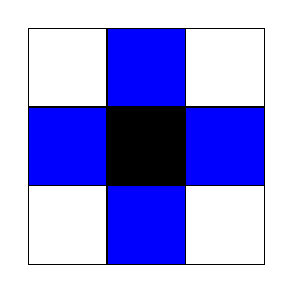
\begin{tikzpicture}
    %Primary node
    \draw[fill=black] (0, 0) rectangle ( 1, 1);

    %Left side
    \draw (-1,-1) rectangle ( 0, 0);
    \draw[fill=blue] (-1, 0) rectangle ( 0, 1);
    \draw (-1, 1) rectangle ( 0, 2);

    %Top
    \draw[fill=blue] ( 0, 1) rectangle ( 1, 2);
    \draw ( 1, 1) rectangle ( 2, 2);

    %Right
    \draw[fill=blue] ( 1, 0) rectangle ( 2, 1);
    \draw ( 1,-1) rectangle ( 2, 0);

    %Bottom
    \draw[fill=blue] ( 0,-1) rectangle ( 1, 0);
  \end{tikzpicture}
\end{document}